\documentclass[a4paper,12pt]{article}
\usepackage[left=2cm,right=2cm,top=2cm,bottom=2cm]{geometry}
\usepackage{tikz}


\title{TikZ commends tutorial}
\date{\today}
\author{Yi-Chen Zhang}

\begin{document}
\maketitle
The TikZ commands can be inside the environment \textbackslash begin\{tikzpicture\} \ldots \textbackslash end\{tikzpicture\} or simply use \textbackslash tikz clause. We run \textsf{pdflatex} or \textsf{latex} followed by \textsf{dvips} to execute the TikZ commends. 

\section{Preliminary}
\subsection{Straight Path Construction}
%Let's get started with drawing a path. A path is a series of straight lines and curves that are connected. We start a path by specifying the coordinates of the start position as a point in brackets, as in $(0,0)$. The starting point is followed by a series of path extension operators `\textsf{-}\textsf{-}'. Then it must be followed by another coordinate and extends the path in a straight line to a new position. We can put some options in square brackets to describe the properties of the lines. This will be discussed later.
\begin{verbatim}
Useage:
  \draw[options] (x1,y1) -- (x2,y2) -- (x3,y3);
\end{verbatim}

\begin{verbatim}
Example:
  \draw (-1.5,0) -- (1.5,0) -- (0,-1.5) -- (0,1.5);
  \draw[thick, rounded corners=10pt] 
    (0,0) -- (0,2) -- (1,3.25) -- (2,2) -- (2,0) -- (0,2) -- (2,2) -- (0,0) -- (2,0);
\end{verbatim}

\tikz \draw (-1.5,0) -- (1.5,0) -- (0,-1.5) -- (0,1.5);
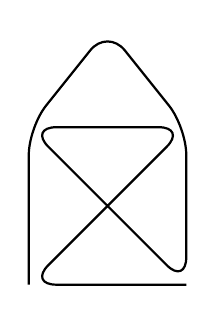
\begin{tikzpicture}
  \draw[thick, rounded corners=10pt] (0,0) -- (0,2) -- (1,3.25) -- (2,2) -- (2,0) -- (0,2) -- (2,2) -- (0,0) -- (2,0); % -- cycle;
\end{tikzpicture}

\subsection{Circle Path Construction}
\begin{verbatim}
Usage:
  \draw[options] (x,y) circle (raidus)
  \draw[options] (x,y) ellipse (raidus1 and radius2)
\end{verbatim}

\begin{verbatim}
Example:
  \draw (0,0) circle (2pt);
  \draw[red] (1,0) circle (3pt);
  \draw[fill=red] (2,0) circle (4pt);
  \draw[red,fill=red] (3,0) circle (5pt);
  \filldraw[blue,rotate=30] (3.5,-2) ellipse (10pt and 5pt);
\end{verbatim}


\begin{tikzpicture}
  \draw (0,0) circle (2pt);
  \draw[red] (1,0) circle (3pt);
  \draw[fill=red] (2,0) circle (4pt);
  \draw[red,fill=red] (3,0) circle (5pt);
  \filldraw[blue,rotate=30] (3.5,-2) ellipse (10pt and 5pt);
\end{tikzpicture}

\end{document}
